\documentclass{article}
\usepackage{amsmath}
\usepackage{listings}
\usepackage[utf8]{inputenc}
\usepackage{graphicx}

\graphicspath{{../results/}}

\lstset{
	basicstyle=\footnotesize,
	numbers=left,
	tabsize=3,
	title=\lstname,
	breaklines=true
}

\addtolength{\oddsidemargin}{-.875in}
\addtolength{\evensidemargin}{-.875in}
\addtolength{\textwidth}{1.75in}

\addtolength{\topmargin}{-.875in}
\addtolength{\textheight}{1.75in}

\title{Neuronale Netze - Übung 6}
\author{Tobias Hahn\\ 3073375}	
	
\begin{document}
\maketitle
\newpage
\section{Erwartungswert \& Hauptkomponenten}
\subsection{Verständnisfrage}
Um herauszubekommen wie viele Punkte gebraucht werden müssen wir zuerst die Anzahl der Regionen ausrechnen, die man mit zwei Hyperebenen abtrennen kann. Die Formel dafür ist (m ist die Anzahl der Hyperebenen, n ist die Dimensionalität der Daten)
\[
 \text{Anzahl Regionen} = 2 * \sum_{i=0}^{n-1}{(\binom{m-1}{i})} 
\]
Für unser Beispiel beträgt die Anzahl der Regionen 4. Jedoch können wir die Aufgabenstellung noch schwieriger machen, indem wir die Punkte einfach auf einer Linie, also in einer Dimension anordnen. Dies ist erlaubt, da wir beliebige Punkte im R2 nehmen können. Dann beträgt die Anzahl der Regionen die wir abtrennen können 3. Wir brauchen dann vier Punkte um sie so anordnen zu können dass sie nicht mehr trennbar sind, auf einer Linie in folgender Abfolge angeordnet: Schwarz, Weiß, Schwarz, Weiß.

\subsection{Programmieraufgabe}
Die Hauptkomponenten wurden in einem Netz mit Ojas Algorithmus berechnet. Der Code und die Ergebnisse hier:

\paragraph{}
Im folgenden zuerst der Quellcode für die beiden Klassen, danach zwei Bilder der Ergebnisse.
\paragraph{}
\lstinputlisting[language=Python]{../meta.py}
\lstinputlisting[language=Python]{../train.py}

\begin{figure}[h]
\caption{Für alle Ziffernklassen: Oben Erwartungswert, danach erste bis neunte Hauptkomponente}
\centering
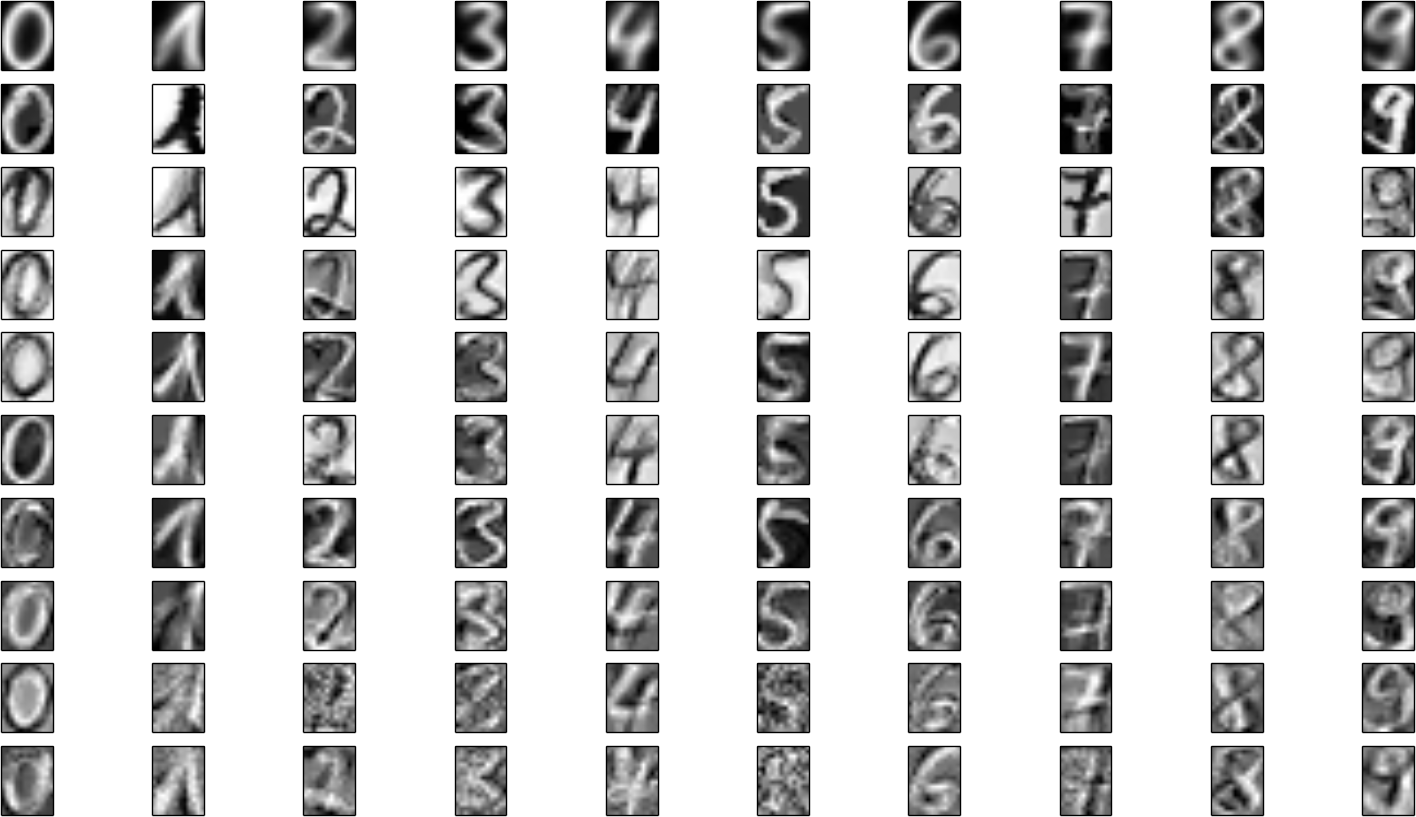
\includegraphics[width=\textwidth]{klassen}
\end{figure}

\begin{figure}[h]
\caption{Für alle Ziffern: Links Erwartungswert, danach erste bis fünfzehnte Hauptkomponente}
\centering
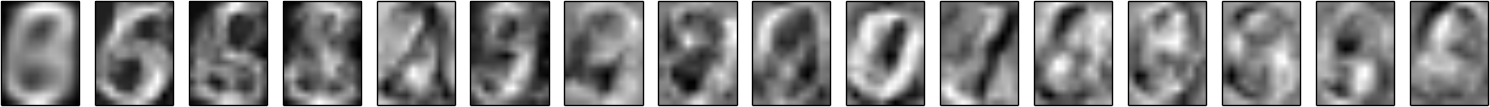
\includegraphics[width=\textwidth]{all_digits}
\end{figure}

\end{document}
